\chapter{Elektronik}

\renewcommand{\kapitelautor}{Autor: Lucas Ullrich}

\begin{figure}[tbh]
\begin{centering}
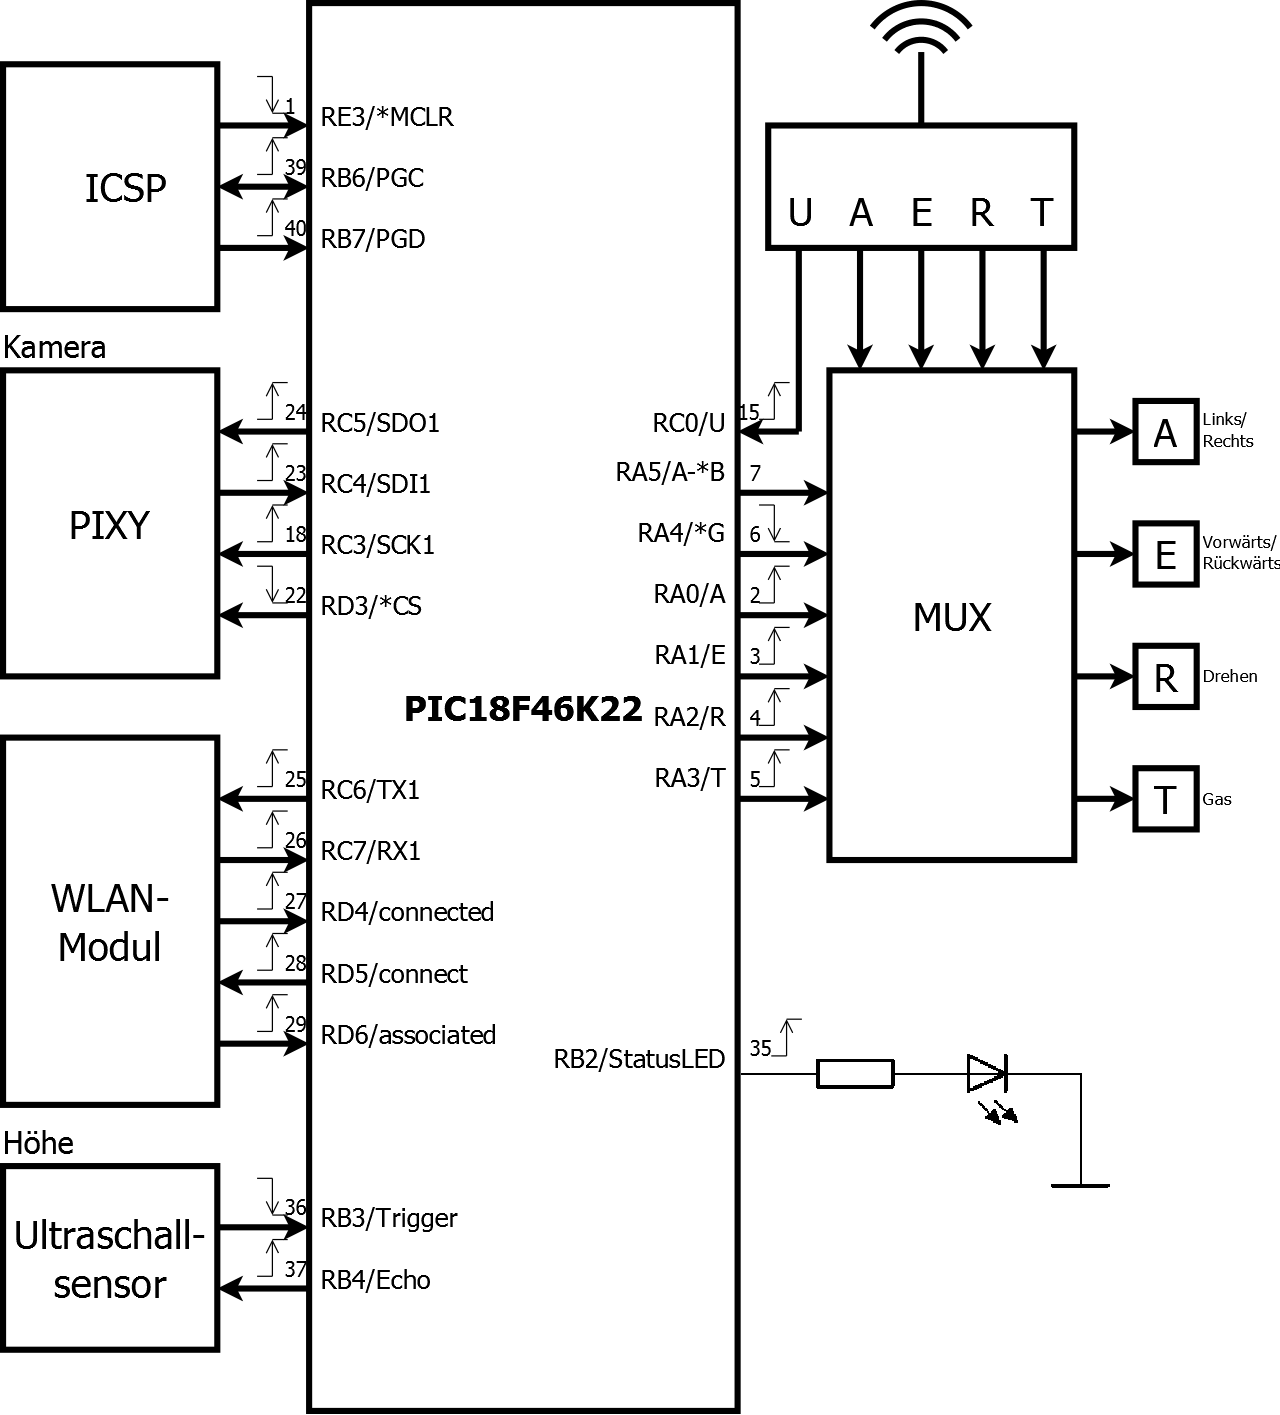
\includegraphics[width = 0.9\textwidth]{Bilder/Blockbild}
\par\end{centering}
\caption{Blockschaltbilder der Hauptplatine}
\label{Blockschaltbild}
\end{figure}

\needspace{3cm}
\section{Sensoren}
Um einen autonomen Flug zu realisieren sind unterschiedliche Sensoren notwendig.
Durch die Sensoren muss es möglich sein die aktuelle Flugposition im Raum zu bestimmen und so den richtigen Weg zu finden.

\subsection{Kamera}
Aufgrund der Zuverlässigkeit einer Kamera im Vergleich zu Systemen die auf Distanzmessungen basieren wurde für die generelle Wegfindung das Kameramodul PIXY cmucam5 gewählt. Dieses gibt die notwendigen Informationen bereits fertig ausgewertet aus. Es wird ein Objektcode, dessen Position auf dem Bild sowie die Objektgröße wiedergegeben.
Anhand dieser Informationen und einer vorher zugesendeten Route kann der Weg zum Ziel bestimmt werden.

\begin{figure}[tbh]
\begin{centering}
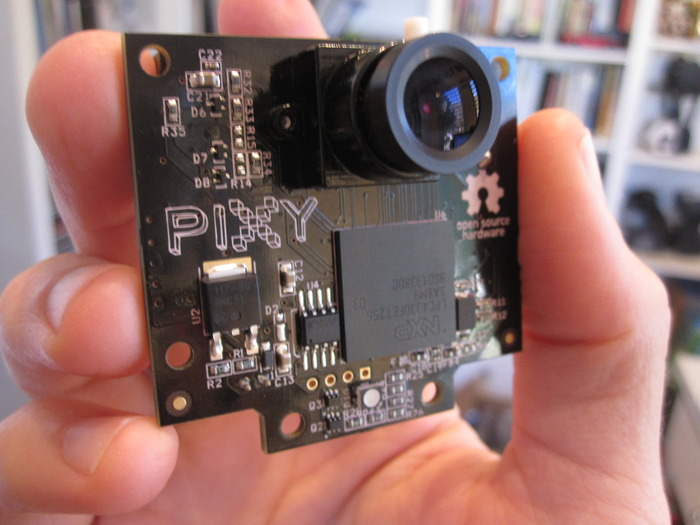
\includegraphics[width = 70mm]{Bilder/PIXY}
\par\end{centering}
\caption{Kamera PIXY cmucam5}
\label{PIXY}
\end{figure}

\subsection{Ultraschallsensor}
Da das Bestimmen der Flughöhe durch die Kamera zwar möglich ist, sich aber sehr aufwändig gestaltet, es müssen diverse Objektparameter bekannt sein und es besteht ein hoher Rechenaufwand, wird für die Messung der FLughöhe ein Ultraschallsensor verwendet. Dieser bietet die Möglichkeit die Flughöhe auf eine Distanz von bis zu 3 m zu bestimmen.